\chapter{Evaluation} \label{chap:Evaluation}
The evaluation of this work has two objectives. First, to make sure that the modified designs still produce correct output. Meaning that the result of an operation when decrypted is the same for both the modified and unmodified versions of the library. Secondly, to profile each design and compare run times of the modified libraries to the unmodified library. 

Distributed systems achieve the best efficiency when working on large inputs. This is because there is some overhead associated with setting up and distributing work. For GPU designs, this overhead time happens when transferring the data to and from the GPU. For distributed computing designs, the overhead time is also in the memory transfers like the GPU, but instead of transferring to the GPU, the memory transfers are between machines. This overhead costs time, that when working with small inputs, usually takes even longer than the operation to complete. Thus the distributed design causes a run time slow down compared to the serial version. However, when working with large amounts of data, the time saved to complete the operation is so great, that the overhead costs are worth it. This characterization of distributed systems is prevalent for these designs, which will be seen later. For these encryption systems, large input sizes occur when $size\_of\_row$ is large. As discussed in the design chapters, $size\_of\_row$ is the length of the vectors in \verb|map|. To best demonstrate the effect $size\_of\_row$ has on the system, $size\_of\_row$ is steadily increased during the testing, so that its effect on each design can be seen and compared to the original design.

To evaluate these designs a few profiling tools were used, discussed in Section \ref{sec:EvaluationTools}. The test environments used for each design are detailed in Section \ref{sec:TestingEnvironment}. The results for GPUHElib are examined in Section \ref{sec:GPUHElibEvaluationResults}, followed by the results for DistributedHElib in Section \ref{sec:DistributedHElibEvaluationResults}.

\section{Evaluation Tools} \label{sec:EvaluationTools}
The following tools were used to evaluate the correctness of the modified libraries and record run times at various levels in the library.

\subsection{Test Program}
A test program was created based on testing programs provided with the original unmodified version of HElib. This new test program first sets up the ciphertexts that are used during computation. Two ciphertexts are created, both are the integers, $0$ to $ num\_slots\_in\_plaintext$. Three operations were reported. The addition, subtraction, and multiplication of two ciphertexts. The other three operations supported, addition, subtraction, and multiplication of a ciphertext and a number, were not reported, as preliminary tests showed that they displayed similar results to their ciphertext only counterparts. It was decided that for conciseness and to avoid repetition, that they would be left out of this document.

The program requires that the user pass in the $size\_of\_row$ they would like to use, which as discussed above, will be incremented during testing. The test program then performs each operation, checking the decrypted result after each operation to make sure that the results are correct, before moving on. Timing blocks were placed around each operation to record the overall time it took to perform the operation. The timers were printed out after each operation. Lower level timers, discussed below, were reset after each operation, so that the lower level times reported with each operation were only times recorded for that operation.

This test program was compiled twice, first linking against the unmodified library, and second against the modified library. This produced two executables, that were then run to generate the results described below.

\subsection{HELib Timing Functions}
The standard version of HElib provides fine grained timing functions that can be placed anywhere throughout the library. To utilized these functions is simple. First a timer is created. Upon the creation of the timer, it is started. A call to \verb|stop| is made in code when the timer should stop. A timer can be started and stopped multiple times, and the average time will be recorded. The timers are stored in a map, and can be reset if needed. This setup allows for fine grained measurement of functions and detailed profiling of run times. 

Each design, serial HElib, GPUHElib, and DistributedHElib required the timers be placed at some similar places, for comparison purposes, and some distinct places, in order to assess the efficiency of each unique design.

\subsubsection{Serial HElib Timer Placement}
There were two levels at which timers were placed, with each successive level more fine grained. The first level was in the test function, described above. This is the circuit level. The other timer was placed at the function level, inside the function that performed the operations in \verb|DoubleCRT|. This function was where the double \verb|for| loop was located that both of the distributed designs are trying to improve upon.

\subsubsection{GPUHElib Timer Placement}
For GPUHElib, there were three levels at which timers were placed. As described above, the first timer was placed at the circuit level in the test program. This would record the time the entire operation took. The second level of timing was the function level. At this level a timer was placed in the function that is performing the operations in \verb|DoubleCRT|. The third and lowest level is the phase level. Four timers are placed at this level to record the setup (vector and stream creation), phase one (host to device memory transfer), phase two (GPU computation), and phase three (device to host memory transfer) times.

\subsubsection{DistributedHElib Timer Placement}
TODO

\section{Testing Environment} \label{sec:TestingEnvironment}
Both systems required unique testing environments that had the capabilities needed for each design. Both variants used machines with 64-bit Intel Core 2 Duo CPUs running at 3.0 Ghz with about 4 Gb of DDR2, 800 Mhz RAM.

\subsection{GPU Testing Environment}
GPUHElib was tested on a machine with a NVIDIA Quadro NVS 290 GPU, which has 256 MB of RAM. Also this particular GPU only has one copy engine. Thus the tests reported here are using the 2-Way Pipelining design discussed in Section \ref{sec:Pipelining}. CUDA version 6.5 was used.

\subsection{Distributed Computing Testing Environment}
DistributedHElib was tested on a cluster of machines all connected through Ethernet. OpenMPI version TODO was used.

\section{GPUHElib Evaluation Results} \label{sec:GPUHElibEvaluationResults}
As discussed earlier in this chapter, the GPU has three levels of timing information begin recorded. The first, and highest level, is the circuit level, where the high level operation is being computed. The second level is the function level, inside \verb|DoubleCRT| where the \verb|parts| are being operated on. And the lowest level is the phase level, where timing results are recorded for all four phases of the operation. The timing results for each of these levels is discussed in more detail in the following sections.

\subsection{Circuit Level Run Time}
\begin{table}[p]
\centering
\begin{tabular}{ | r | r | r | r | r | r | r | }
 \multicolumn{1}{ r }{} & \multicolumn{6}{ c }{$size\_of\_row$} \\ \cline{2-7}
 \multicolumn{1}{ r |}{} & $1{,}000$ & $10{,}000$ & $100{,}000$ & $200{,}000$ & $300{,}000$ & $400{,}000$ \\ \hline
 Add & 1.400E-05 & 1.080E-04 & 2.545E-03 & 5.396E-03 & 5.354E-03 & 1.053E-02 \\ \hline
 Sub & 1.400E-05 & 1.300E-04 & 2.532E-03 & 5.304E-03 & 5.366E-03 & 1.075E-02 \\ \hline
 Mul & 4.962E-03 & 1.036E-01 & 1.157 & 2.648 & 7.217 & 1.232E+01 \\ \hline
\end{tabular}
\caption{Serial HElib circuit level run times (in seconds)}
\label{tab:serialLevel1Runtimes}
\end{table}

\begin{table}[p]
\centering
\begin{tabular}{ | r | r | r | r | r | r | r | }
 \multicolumn{1}{ r }{} & \multicolumn{6}{ c }{$size\_of\_row$} \\ \cline{2-7}
 \multicolumn{1}{ r |}{} & $1{,}000$ & $10{,}000$ & $100{,}000$ & $200{,}000$ & $300{,}000$ & $400{,}000$ \\ \hline
 Add & 1.050E-03 & 1.675E-03 & 8.972E-03 & 1.646E-02 & 1.671E-02 & 3.704E-02 \\ \hline
 Sub & 1.012E-03 & 1.805E-03 & 9.023E-03 & 1.683E-02 & 1.682E-02 & 3.700E-02 \\ \hline
 Mul & 1.106E-02 & 1.187E-01 & 1.309 & 2.868 & 7.393 & 9.333 \\ \hline
\end{tabular}
\caption{GPUHElib circuit level run times (in seconds)}
\label{tab:GPULevel1Runtimes}
\end{table}

\begin{figure}[p]
\centering

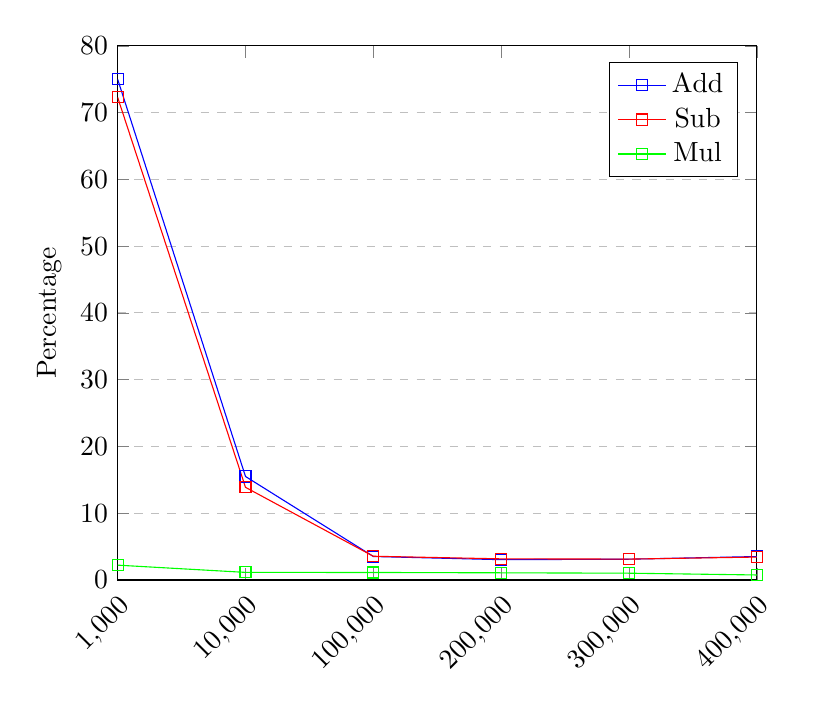
\begin{tikzpicture}
\begin{axis}
[
    ylabel={Percentage},
    width=.8\textwidth,
    xmin=1, xmax=6,
    ymin=0, ymax=80,
    xtick={1,2,3,4,5,6},
    xticklabels={$1{,}000$, $10{,}000$, $100{,}000$, $200{,}000$, $300{,}000$, $400{,}000$},
    ytick={80,70,60,50,40,30,20,10,0},
    legend pos=north east,
    ymajorgrids=true,
    grid style=dashed,
    x tick label style={rotate=45,anchor=north east},
]

\addplot[color=blue,mark=square]
    coordinates {
    (1,75)(2,15.50925926)(3,3.525343811)(4,3.049481097)(5,3.121404557)(6,3.519144893) };
    
\addplot[color=red,mark=square]
    coordinates {
    (1,72.28571429)(2,13.88461538)(3,3.563586098)(4,3.172511312)(5,3.1339918)(6,3.441354293) };

\addplot[color=green,mark=square]
    coordinates {
    (1,2.229544538)(2,1.146005137)(3,1.131587363)(4,1.083041024)(5,1.024489643)(6,0.757830934) };
    
\legend{Add,Sub,Mul}
 
\end{axis}
\end{tikzpicture}

\caption{Run Time Comparison at Circuit Level}
\label{fig:level1ComparisonSerialGPU}
\end{figure}

Table \ref{tab:serialLevel1Runtimes} and Table \ref{tab:GPULevel1Runtimes} display the run times for serial HElib and GPUHElib tests respectively. Both tests were run with inputs sizes starting at 1,000 and increasing until 400,000. Figure \ref{fig:level1ComparisonSerialGPU} visualizes these times as the slowdown of GPUHElib over serial HElib. A value of 1 means that the serial version and the GPU version had the same run time. Above 1 means that the GPU design has a slower run time, and below 1 means that the GPU has a faster run time.

One can see in Figure \ref{fig:level1ComparisonSerialGPU} that for the smaller input sizes, the run times for the GPU are much larger than the serial version for addition and subtraction. They start off taking about 72 times as long to complete compared to the serial version. The multiplication operation also starts off taking longer, however only about 2.2 times as long. The run times for serial HElib and GPUHElib get closer and closer, as the inputs sizes approach 400,000. The addition and subtraction circuit run times minimize at about 3 times as long, for the 300,000 size input. However for the 400,000 size input, the times go in the opposite direction desired, becoming about 3.5 times as long. The multiplication circuit actually has the best results, with the 400,000 test taking about .75 times the serial version. So the multiplication circuit took about 3/4 the time to complete in GPUHElib compared to the serial version. While this result might look good, further analysis of the lower level tests show that this was probably not caused by the usage of the GPU, but by other operations computed during the multiplication operation being faster. The function level run times will be examined next.

\subsection{Function Level Run Time}
\begin{table}[p]
\centering
\begin{tabular}{ | r | r | r | r | r | r | r | }
 \multicolumn{1}{ r }{} & \multicolumn{6}{ c }{$size\_of\_row$} \\ \cline{2-7}
 \multicolumn{1}{ r |}{} & $1{,}000$ & $10{,}000$ & $100{,}000$ & $200{,}000$ & $300{,}000$ & $400{,}000$ \\ \hline
 Add & 5.000E-06 & 4.825E-05 & 1.007E-03 & 2.648E-03 & 2.653E-03 & 5.466E-03 \\ \hline
 Sub & 5.000E-06 & 6.150E-05 & 1.259E-03 & 2.644E-03 & 2.674E-03 & 5.366E-03 \\ \hline
 Mul & 2.900E-05 & 2.830E-04 & 2.879E-03 & 5.863E-03 & 5.856E-03 & 1.176E-02 \\ \hline
\end{tabular}
\caption{Serial HElib function level run times (in seconds)}
\label{tab:serialLevel2Runtimes}
\end{table}

\begin{table}[p]
\centering
\begin{tabular}{ | r | r | r | r | r | r | r | }
 \multicolumn{1}{ r }{} & \multicolumn{6}{ c }{$size\_of\_row$} \\ \cline{2-7}
 \multicolumn{1}{ r |}{} & $1{,}000$ & $10{,}000$ & $100{,}000$ & $200{,}000$ & $300{,}000$ & $400{,}000$ \\ \hline
 Add & 5.210E-04 & 8.298E-04 & 4.392E-03 & 8.257E-03 & 8.346E-03 & 1.864E-02 \\ \hline
 Sub & 5.020E-04 & 8.950E-04 & 4.498E-03 & 8.398E-03 & 8.395E-03 & 1.848E-02 \\ \hline
 Mul & 5.302E-04 & 1.006E-03 & 6.599E-03 & 1.273E-02 & 1.276E-02 & 2.687E-02 \\ \hline
\end{tabular}
\caption{GPUHElib function level run times (in seconds)}
\label{tab:GPULevel2Runtimes}
\end{table}

\begin{figure}[p]
\centering
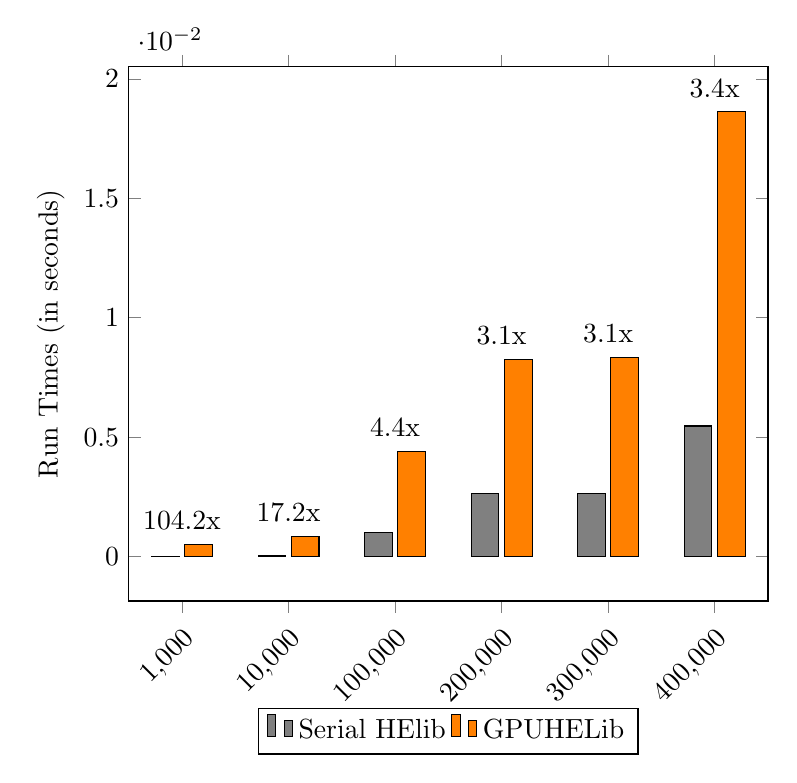
\begin{tikzpicture}

\begin{axis}[
    ybar,
    width=.8\textwidth,
    legend style={at={(0.5,-0.2)},anchor=north,legend columns=-1},
    ylabel=Run Times (in seconds),
    symbolic x coords={$1{,}000$,$10{,}000$,$100{,}000$,$200{,}000$,$300{,}000$,$400{,}000$},
    xtick=data,
    x tick label style={rotate=45,anchor=north east},
]

\addplot[fill=gray]
    coordinates {
    ($1{,}000$,5.000E-06)($10{,}000$,4.825E-05)($100{,}000$,1.007E-03)($200{,}000$,2.648E-03)($300{,}000$,2.653E-03)($400{,}000$,5.466E-03) };
    
\addplot[fill=orange]
    coordinates {
    ($1{,}000$,5.210E-04)($10{,}000$,8.298E-04)($100{,}000$,4.392E-03)($200{,}000$,8.257E-03)($300{,}000$,8.346E-03)($400{,}000$,1.864E-02) };
    
\node at (axis cs:$1{,}000$,1.52E-03) {104.2x};
\node at (axis cs:$10{,}000$,1.83E-03) {17.2x};
\node at (axis cs:$100{,}000$,5.39E-03) {4.4x};
\node at (axis cs:$200{,}000$,9.26E-03) {3.1x};
\node at (axis cs:$300{,}000$,9.35E-03) {3.1x};
\node at (axis cs:$400{,}000$,1.96E-02) {3.4x};
    
\legend{Serial HElib,GPUHELib}
\end{axis}
\end{tikzpicture}

\caption{Add Run Times Comparison at Function Level}
\label{fig:level2ComparisonSerialGPUAddVecs}
\end{figure}

\begin{figure}[p]
\centering
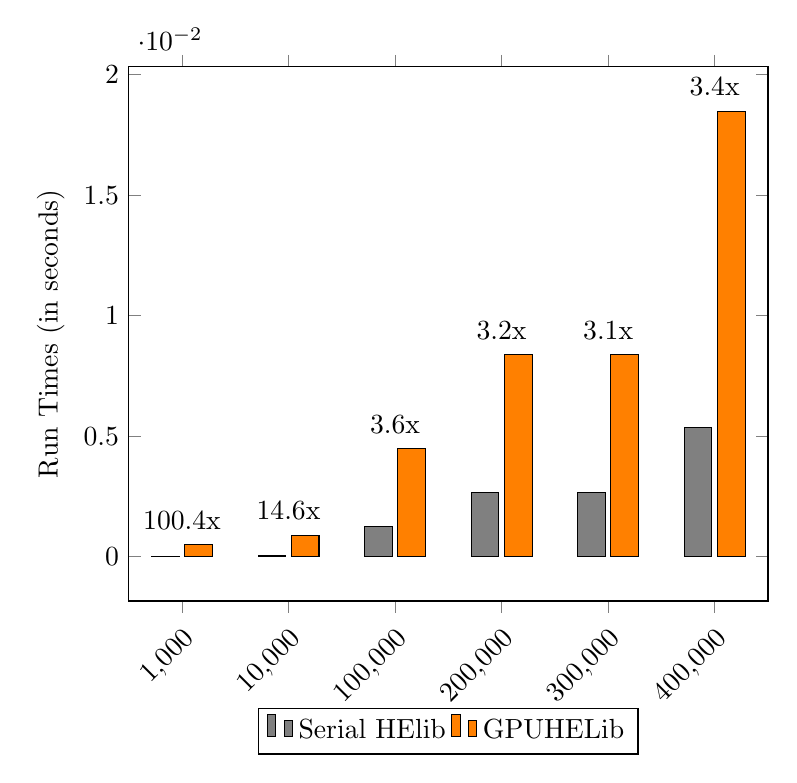
\begin{tikzpicture}

\begin{axis}[
    ybar,
    width=.8\textwidth,
    legend style={at={(0.5,-0.2)},anchor=north,legend columns=-1},
    ylabel=Run Times (in seconds),
    symbolic x coords={$1{,}000$,$10{,}000$,$100{,}000$,$200{,}000$,$300{,}000$,$400{,}000$},
    xtick=data,
    x tick label style={rotate=45,anchor=north east},
]

\addplot[fill=gray]
    coordinates {
    ($1{,}000$,5.000E-06)($10{,}000$,6.150E-05)($100{,}000$,1.259E-03)($200{,}000$,2.644E-03)($300{,}000$,2.674E-03)($400{,}000$,5.366E-03) };
    
\addplot[fill=orange]
    coordinates {
    ($1{,}000$,5.020E-04)($10{,}000$,8.950E-04)($100{,}000$,4.498E-03)($200{,}000$,8.398E-03)($300{,}000$,8.395E-03)($400{,}000$,1.848E-02) };

\node at (axis cs:$1{,}000$,1.50E-03) {100.4x};
\node at (axis cs:$10{,}000$,1.90E-03) {14.6x};
\node at (axis cs:$100{,}000$,5.50E-03) {3.6x};
\node at (axis cs:$200{,}000$,9.40E-03) {3.2x};
\node at (axis cs:$300{,}000$,9.39E-03) {3.1x};
\node at (axis cs:$400{,}000$,1.95E-02) {3.4x};
    
\legend{Serial HElib,GPUHELib}
\end{axis}
\end{tikzpicture}

\caption{Sub Run Times Comparison at Function Level}
\label{fig:level2ComparisonSerialGPUSubVecs}
\end{figure}

\begin{figure}[p]
\centering
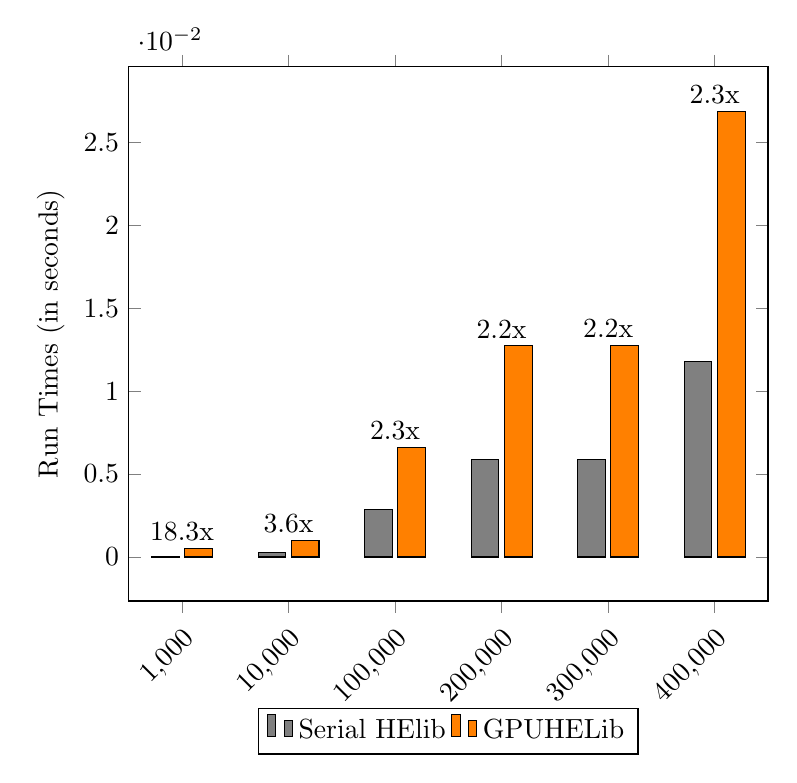
\begin{tikzpicture}

\begin{axis}[
    ybar,
    width=.8\textwidth,
    legend style={at={(0.5,-0.2)},anchor=north,legend columns=-1},
    ylabel=Run Times (in seconds),
    symbolic x coords={$1{,}000$,$10{,}000$,$100{,}000$,$200{,}000$,$300{,}000$,$400{,}000$},
    xtick=data,
    x tick label style={rotate=45,anchor=north east},
]

\addplot[fill=gray]
    coordinates {
    ($1{,}000$,2.900E-05)($10{,}000$,2.830E-04)($100{,}000$,2.879E-03)($200{,}000$,5.863E-03)($300{,}000$,5.856E-03)($400{,}000$,1.176E-02) };
    
\addplot[fill=orange]
    coordinates {
    ($1{,}000$,5.302E-04)($10{,}000$,1.006E-03)($100{,}000$,6.599E-03)($200{,}000$,1.273E-02)($300{,}000$,1.276E-02)($400{,}000$,2.687E-02) };
    					
\node at (axis cs:$1{,}000$,1.53E-03) {18.3x};
\node at (axis cs:$10{,}000$,2.01E-03) {3.6x};
\node at (axis cs:$100{,}000$,7.60E-03) {2.3x};
\node at (axis cs:$200{,}000$,1.37E-02) {2.2x};
\node at (axis cs:$300{,}000$,1.38E-02) {2.2x};
\node at (axis cs:$400{,}000$,2.79E-02) {2.3x};
    
\legend{Serial HElib,GPUHELib}
\end{axis}
\end{tikzpicture}

\caption{Mul Run Times Comparison at Function Level}
\label{fig:level2ComparisonSerialGPUMulVecs}
\end{figure}

Table \ref{tab:serialLevel2Runtimes} and Table \ref{tab:GPULevel2Runtimes} display the run times for the serial HElib and GPUHElib tests respectively. As noted before, both tests were run with input sizes ranging from 1,000 to 400,000.

Figure \ref{fig:level2ComparisonSerialGPUAddVecs}, Figure \ref{fig:level2ComparisonSerialGPUSubVecs}, and Figure \ref{fig:level2ComparisonSerialGPUMulVecs} show the comparisons between the run times for each of the operations at the function level. Also displayed in the figures is the run time slow down of the GPU variant compared to the serial version. So, for example, in Figure \ref{fig:level2ComparisonSerialGPUAddVecs}, the 104.2x above 1,000 means that the GPU variant took 104.2 times longer to complete compared to the serial version.

All these times again reiterate that for the smaller input sizes, the run times for the GPU variant are vastly larger, almost 100x for addition and subtraction, and about 18x for multiplication. As the input sizes increase, the run times get closer and closer, but minimize at about 3.1x for addition and subtraction and at about 2x for multiplication. Again one can see that for the 400,000 input size, the slow downs increase for all the operations compared to the previous input size, 300,000, going from 3.2x to 3.4x and 3.5x respectively and from 2.2x to 2.3x. The results for the multiplication times make it clear that the speedup seen at the circuit level must be cause my other factors than the GPU implementation of multiplication. These times show that multiplication behaves exactly like the other operations in terms of run time patterns. The cause for these slow downs is evident after examining the recorded times at the phase level.

\subsection{Phase Level Run Time}
\begin{table}[p]
\centering
\begin{tabular}{ | r | r | r | r | r | r | r | }
 \multicolumn{1}{ r }{} & \multicolumn{6}{ c }{$size\_of\_row$} \\ \cline{2-7}
 \multicolumn{1}{ r |}{} & $1{,}000$ & $10{,}000$ & $100{,}000$ & $200{,}000$ & $300{,}000$ & $400{,}000$ \\ \hline
 Setup & 2.420E-04 & 2.465E-04 & 2.848E-04 & 3.013E-04 & 3.015E-04 & 3.133E-04 \\ \hline
 Phase 1 & 9.500E-05 & 2.568E-04 & 2.137E-03 & 4.289E-03 & 4.345E-03 & 1.164E-02 \\ \hline
 Phase 2 & 4.425E-05 & 3.350E-05 & 1.283E-04 & 2.423E-04 & 2.420E-04 & 3.728E-04 \\ \hline
 Phase 3 & 1.373E-04 & 2.900E-04 & 1.837E-03 & 3.420E-03 & 3.454E-03 & 6.308E-03 \\ \hline
\end{tabular}
\caption{GPUHElib Add phase level run times (in seconds)}
\label{tab:GPULevel3RuntimesAddVecs}
\end{table}

\begin{figure}[p]
\centering
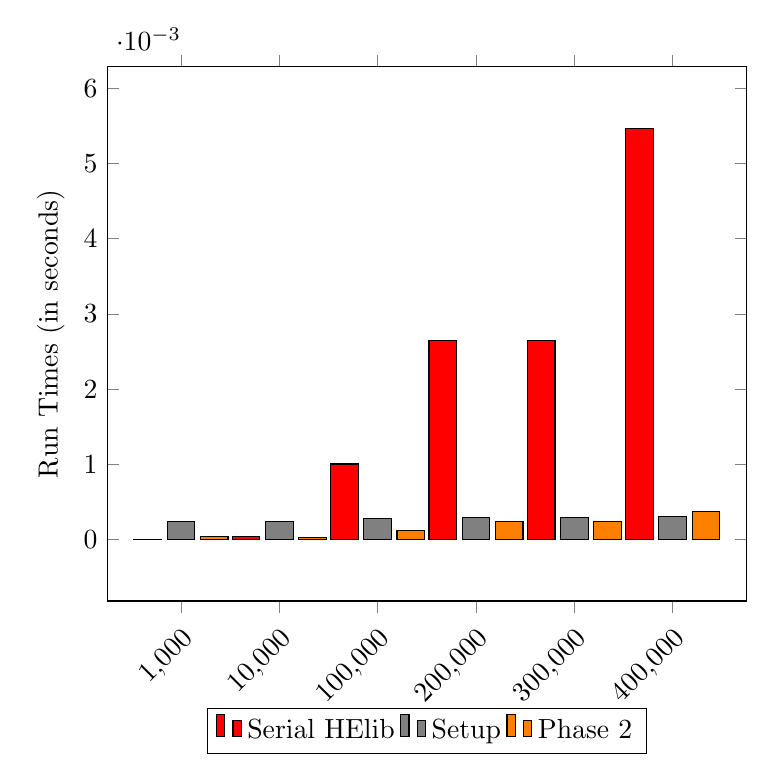
\begin{tikzpicture}

\begin{axis}[
    ybar,
    width=.8\textwidth,
    enlargelimits=0.15,
    legend style={at={(0.5,-0.2)},anchor=north,legend columns=-1},
    ylabel=Run Times (in seconds),
    symbolic x coords={$1{,}000$,$10{,}000$,$100{,}000$,$200{,}000$,$300{,}000$,$400{,}000$},
    xtick=data,
    x tick label style={rotate=45,anchor=north east},
]

\addplot[fill=red]
    coordinates {
    ($1{,}000$,5.000E-06)($10{,}000$,4.825E-05)($100{,}000$,1.007E-03)($200{,}000$,2.648E-03)($300{,}000$,2.653E-03)($400{,}000$,5.466E-03) };
    
\addplot[fill=gray]
    coordinates {
    ($1{,}000$,2.420E-04)($10{,}000$,2.465E-04)($100{,}000$,2.848E-04)($200{,}000$,3.013E-04)($300{,}000$,3.015E-04)($400{,}000$,3.133E-04) };
    
\addplot[fill=orange]
    coordinates {
    ($1{,}000$,4.425E-05)($10{,}000$,3.350E-05)($100{,}000$,1.283E-04)($200{,}000$,2.423E-04)($300{,}000$,2.420E-04)($400{,}000$,3.728E-04) };
    
\legend{Serial HElib,Setup,Phase 2}
\end{axis}
\end{tikzpicture}

\caption{Add Phase Level Run Times Comparison - Operation}
\label{fig:level3ComparisonSerialGPUAddVecs1}
\end{figure}

\begin{figure}[p]
\centering
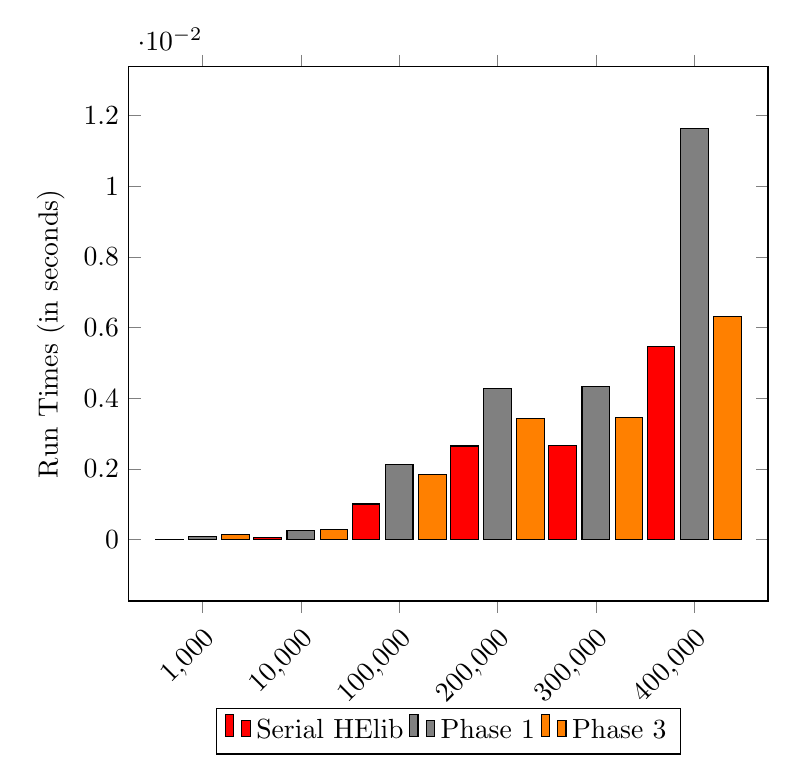
\begin{tikzpicture}

\begin{axis}[
    ybar,
    width=.8\textwidth,
    enlargelimits=0.15,
    legend style={at={(0.5,-0.2)},anchor=north,legend columns=-1},
    ylabel=Run Times (in seconds),
    symbolic x coords={$1{,}000$,$10{,}000$,$100{,}000$,$200{,}000$,$300{,}000$,$400{,}000$},
    xtick=data,
    x tick label style={rotate=45,anchor=north east},
]

\addplot[fill=red]
    coordinates {
    ($1{,}000$,5.000E-06)($10{,}000$,4.825E-05)($100{,}000$,1.007E-03)($200{,}000$,2.648E-03)($300{,}000$,2.653E-03)($400{,}000$,5.466E-03) };
    
\addplot[fill=gray]
    coordinates {
    ($1{,}000$,9.500E-05)($10{,}000$,2.568E-04)($100{,}000$,2.137E-03)($200{,}000$,4.289E-03)($300{,}000$,4.345E-03)($400{,}000$,1.164E-02) };
    
\addplot[fill=orange]
    coordinates {
    ($1{,}000$,1.373E-04)($10{,}000$,2.900E-04)($100{,}000$,1.837E-03)($200{,}000$,3.420E-03)($300{,}000$,3.454E-03)($400{,}000$,6.308E-03) };
    
\legend{Serial HElib,Phase 1,Phase 3}
\end{axis}
\end{tikzpicture}

\caption{Add Phase Level Run Times Comparison - Memory}
\label{fig:level3ComparisonSerialGPUAddVecs2}
\end{figure}

\begin{table}[p]
\centering
\begin{tabular}{ | r | r | r | r | r | r | r | }
 \multicolumn{1}{ r }{} & \multicolumn{6}{ c }{$size\_of\_row$} \\ \cline{2-7}
 \multicolumn{1}{ r |}{} & $1{,}000$ & $10{,}000$ & $100{,}000$ & $200{,}000$ & $300{,}000$ & $400{,}000$ \\ \hline
 Setup & 2.455E-04 & 2.830E-04 & 3.035E-04 & 3.065E-04 & 3.045E-04 & 3.050E-04 \\ \hline
 Phase 1 & 9.000E-05 & 2.535E-04 & 2.262E-03 & 4.377E-03 & 4.377E-03 & 1.152E-02 \\ \hline
 Phase 2 & 3.400E-05 & 4.200E-05 & 1.280E-04 & 2.420E-04 & 2.425E-04 & 3.745E-04 \\ \hline
 Phase 3 & 1.275E-04 & 3.120E-04 & 1.799E-03 & 3.466E-03 & 3.465E-03 & 6.275E-03 \\ \hline
\end{tabular}
\caption{GPUHElib Sub phase level run times (in seconds)}
\label{tab:GPULevel3RuntimesSubVecs}
\end{table}

\begin{figure}[p]
\centering
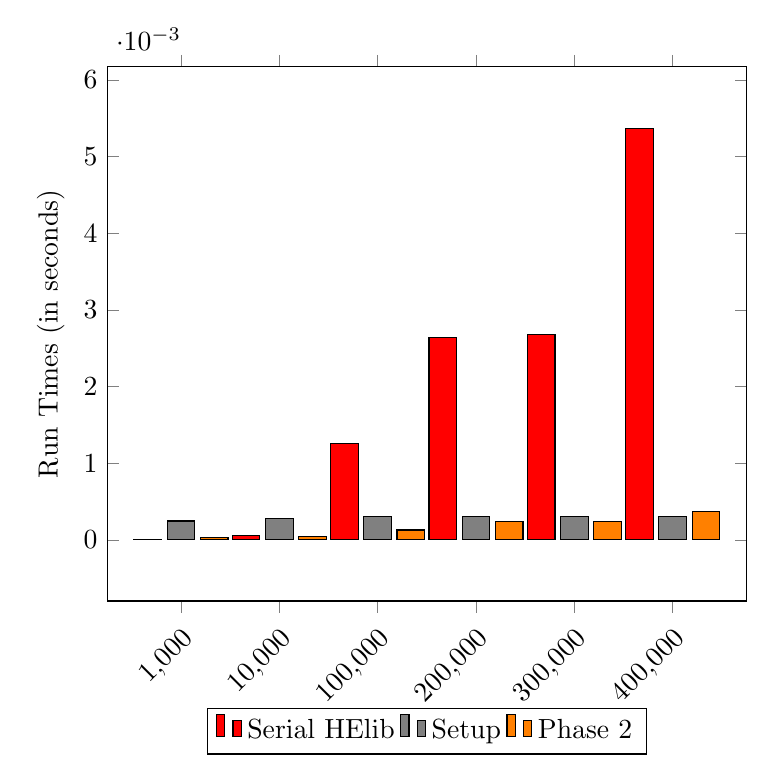
\begin{tikzpicture}

\begin{axis}[
    ybar,
    width=.8\textwidth,
    enlargelimits=0.15,
    legend style={at={(0.5,-0.2)},anchor=north,legend columns=-1},
    ylabel=Run Times (in seconds),
    symbolic x coords={$1{,}000$,$10{,}000$,$100{,}000$,$200{,}000$,$300{,}000$,$400{,}000$},
    xtick=data,
    x tick label style={rotate=45,anchor=north east},
]

\addplot[fill=red]
    coordinates {
    ($1{,}000$,5.000E-06)($10{,}000$,6.150E-05)($100{,}000$,1.259E-03)($200{,}000$,2.644E-03)($300{,}000$,2.674E-03)($400{,}000$,5.366E-03) };
    
\addplot[fill=gray]
    coordinates {
    ($1{,}000$,2.455E-04)($10{,}000$,2.830E-04)($100{,}000$,3.035E-04)($200{,}000$,3.065E-04)($300{,}000$,3.045E-04)($400{,}000$,3.050E-04) };
    
\addplot[fill=orange]
    coordinates {
    ($1{,}000$,3.400E-05)($10{,}000$,4.200E-05)($100{,}000$,1.280E-04)($200{,}000$,2.420E-04)($300{,}000$,2.425E-04)($400{,}000$,3.745E-04) };
    
\legend{Serial HElib,Setup,Phase 2}
\end{axis}
\end{tikzpicture}

\caption{Sub Phase Level Run Times Comparison - Operation}
\label{fig:level3ComparisonSerialGPUSubVecs1}
\end{figure}

\begin{figure}[p]
\centering
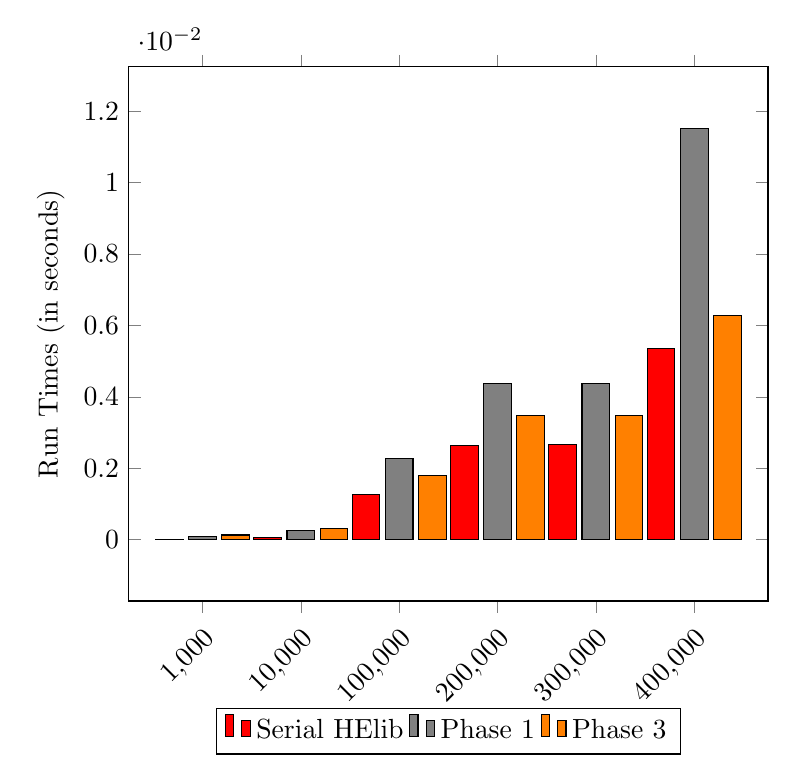
\begin{tikzpicture}

\begin{axis}[
    ybar,
    width=.8\textwidth,
    enlargelimits=0.15,
    legend style={at={(0.5,-0.2)},anchor=north,legend columns=-1},
    ylabel=Run Times (in seconds),
    symbolic x coords={$1{,}000$,$10{,}000$,$100{,}000$,$200{,}000$,$300{,}000$,$400{,}000$},
    xtick=data,
    x tick label style={rotate=45,anchor=north east},
]

\addplot[fill=red]
    coordinates {
    ($1{,}000$,5.000E-06)($10{,}000$,6.150E-05)($100{,}000$,1.259E-03)($200{,}000$,2.644E-03)($300{,}000$,2.674E-03)($400{,}000$,5.366E-03) };
    
\addplot[fill=gray]
    coordinates {
    ($1{,}000$,9.000E-05)($10{,}000$,2.535E-04)($100{,}000$,2.262E-03)($200{,}000$,4.377E-03)($300{,}000$,4.377E-03)($400{,}000$,1.152E-02) };
    
\addplot[fill=orange]
    coordinates {
    ($1{,}000$,1.275E-04)($10{,}000$,3.120E-04)($100{,}000$,1.799E-03)($200{,}000$,3.466E-03)($300{,}000$,3.465E-03)($400{,}000$,6.275E-03) };
    
\legend{Serial HElib,Phase 1,Phase 3}
\end{axis}
\end{tikzpicture}

\caption{Sub Phase Level Run Times Comparison - Memory}
\label{fig:level3ComparisonSerialGPUSubVecs2}
\end{figure}

\begin{table}[p]
\centering
\begin{tabular}{ | r | r | r | r | r | r | r | }
 \multicolumn{1}{ r }{} & \multicolumn{6}{ c }{$size\_of\_row$} \\ \cline{2-7}
 \multicolumn{1}{ r |}{} & $1{,}000$ & $10{,}000$ & $100{,}000$ & $200{,}000$ & $300{,}000$ & $400{,}000$ \\ \hline
 Setup & 2.405E-04 & 2.447E-04 & 3.027E-04 & 3.200E-04 & 3.157E-04 & 3.207E-04 \\ \hline
 Phase 1 & 7.933E-05 & 1.853E-04 & 1.845E-03 & 3.955E-03 & 3.997E-03 & 1.029E-02 \\ \hline
 Phase 2 & 3.000E-05 & 3.183E-05 & 1.247E-04 & 2.398E-04 & 2.353E-04 & 3.508E-04 \\ \hline
 Phase 3 & 1.772E-04 & 5.418E-04 & 4.323E-03 & 8.213E-03 & 8.212E-03 & 1.591E-02 \\ \hline
\end{tabular}
\caption{GPUHElib Mul phase level run times (in seconds)}
\label{tab:GPULevel3RuntimesMulVecs}
\end{table}

\begin{figure}[p]
\centering
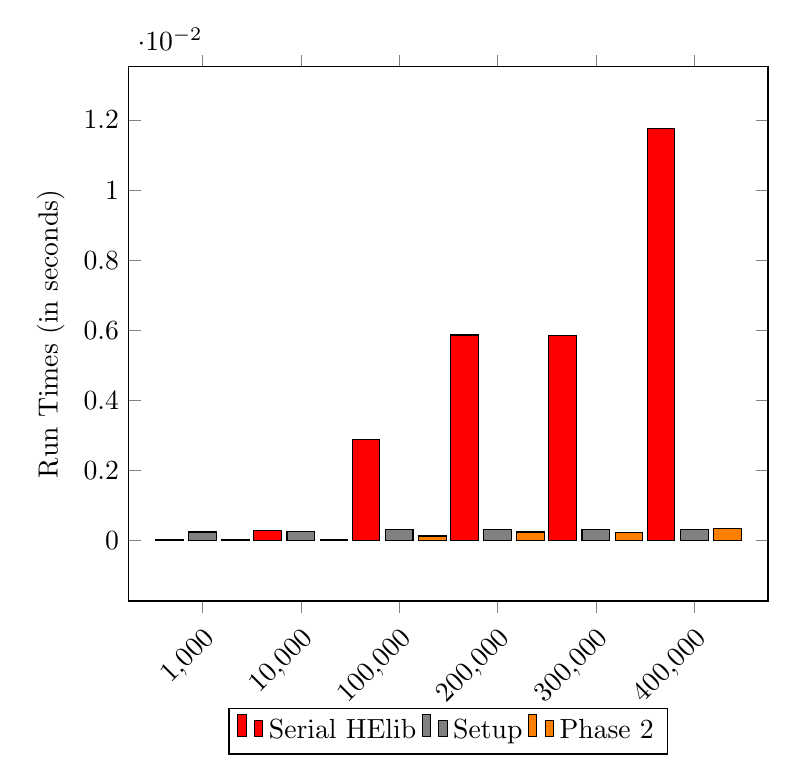
\begin{tikzpicture}

\begin{axis}[
    ybar,
    width=.8\textwidth,
    enlargelimits=0.15,
    legend style={at={(0.5,-0.2)},anchor=north,legend columns=-1},
    ylabel=Run Times (in seconds),
    symbolic x coords={$1{,}000$,$10{,}000$,$100{,}000$,$200{,}000$,$300{,}000$,$400{,}000$},
    xtick=data,
    x tick label style={rotate=45,anchor=north east},
]

\addplot[fill=red]
    coordinates {
    ($1{,}000$,2.900E-05)($10{,}000$,2.830E-04)($100{,}000$,2.879E-03)($200{,}000$,5.863E-03)($300{,}000$,5.856E-03)($400{,}000$,1.176E-02) };
    
\addplot[fill=gray]
    coordinates {
    ($1{,}000$,2.405E-04)($10{,}000$,2.447E-04)($100{,}000$,3.027E-04)($200{,}000$,3.200E-04)($300{,}000$,3.157E-04)($400{,}000$,3.207E-04) };
    
\addplot[fill=orange]
    coordinates {
    ($1{,}000$,3.000E-05)($10{,}000$,3.183E-05)($100{,}000$,1.247E-04)($200{,}000$,2.398E-04)($300{,}000$,2.353E-04)($400{,}000$,3.508E-04) };
    
\legend{Serial HElib,Setup,Phase 2}
\end{axis}
\end{tikzpicture}

\caption{Mul Phase Level Run Times Comparison - Operation}
\label{fig:level3ComparisonSerialGPUMulVecs1}
\end{figure}

\begin{figure}[p]
\centering
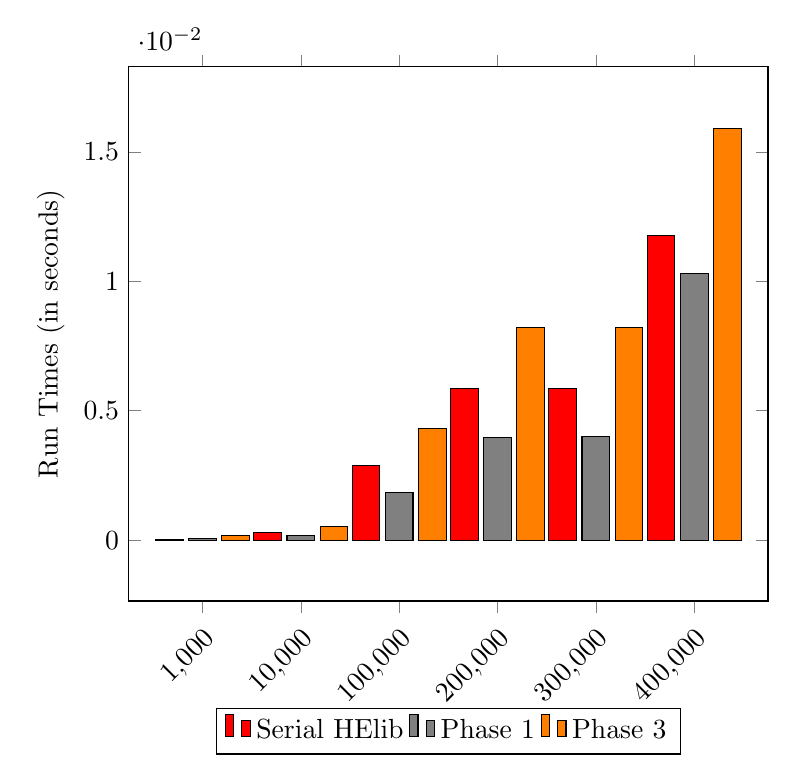
\begin{tikzpicture}

\begin{axis}[
    ybar,
    width=.8\textwidth,
    enlargelimits=0.15,
    legend style={at={(0.5,-0.2)},anchor=north,legend columns=-1},
    ylabel=Run Times (in seconds),
    symbolic x coords={$1{,}000$,$10{,}000$,$100{,}000$,$200{,}000$,$300{,}000$,$400{,}000$},
    xtick=data,
    x tick label style={rotate=45,anchor=north east},
]

\addplot[fill=red]
    coordinates {
    ($1{,}000$,2.900E-05)($10{,}000$,2.830E-04)($100{,}000$,2.879E-03)($200{,}000$,5.863E-03)($300{,}000$,5.856E-03)($400{,}000$,1.176E-02) };
    
\addplot[fill=gray]
    coordinates {
    ($1{,}000$,7.933E-05)($10{,}000$,1.853E-04)($100{,}000$,1.845E-03)($200{,}000$,3.955E-03)($300{,}000$,3.997E-03)($400{,}000$,1.029E-02) };
    
\addplot[fill=orange]
    coordinates {
    ($1{,}000$,1.772E-04)($10{,}000$,5.418E-04)($100{,}000$,4.323E-03)($200{,}000$,8.213E-03)($300{,}000$,8.212E-03)($400{,}000$,1.591E-02) };
    
\legend{Serial HElib,Phase 1,Phase 3}
\end{axis}
\end{tikzpicture}

\caption{Mul Phase Level Run Times Comparison - Memory}
\label{fig:level3ComparisonSerialGPUMulVecs2}
\end{figure}

Table \ref{tab:GPULevel3RuntimesAddVecs}, Table \ref{tab:GPULevel3RuntimesSubVecs}, and Table \ref{tab:GPULevel3RuntimesMulVecs} all display the phase level run times for each operation respectively. The four phases are: setup (vector and stream creation), phase 1 (host to device memory copy), phase 2 (operation on GPU), and phase 3 (device to host memory copy). These times have been split between two plots for each operation. One group of plots focuses on the overall run time of serial HElib compared to the setup and phase 2 times recorded. These are the \say{Operation} plots, Figure \ref{fig:level3ComparisonSerialGPUAddVecs1}, Figure \ref{fig:level3ComparisonSerialGPUSubVecs1}, and Figure \ref{fig:level3ComparisonSerialGPUMulVecs1}. The other group of plots focuses on the overhead phases, phase 1 and phase 3, of GPUHElib compared to the overall run time of serial HElib for each operation and are denoted \say{Memory}. These are Figure \ref{fig:level3ComparisonSerialGPUAddVecs2}, Figure \ref{fig:level3ComparisonSerialGPUSubVecs2}, and Figure \ref{fig:level3ComparisonSerialGPUMulVecs2}.

The \say{Operation} plots show that the design is working as intended and as all GPU designs ideally are suppose to work. The reliance on the GPU to perform the computation drastically reduces the run time for those phases. Furthermore as the input size increases largely, the run times for setup and phase 2 only increase slightly. When the input sizes are small, again the overhead of using the GPU causes the run times to be large compared to the serial version. 

The setup phase always took about the same amount of time no matter the input size, only varying by about 8E-05 from the smallest input to the largest. Phase 2 steadily increased, however not at the rapid degree that the serial version did. This is what is expected when using a GPU to perform operations.

The \say{Memory} plots show where this design fails. The amount of time needed to move the data back and forth from the GPU is immense. The times for phase 1 and phase 3 are always larger than the entire run time of the serial version for every operation across all input sizes, except for the multiplication operation, where the phase 1 times are actually less than the overall run time of the serial version, but not by much. These times are very disappointing, as they are the reason that this design is performing so poorly. Luckily, these times could be lower, given better hardware and possible future work, which could make GPUHElib a viable option. If the problem was in the design or if the run times for the setup or phase 1 were worse, then the total design would not have any hope of being used. But because they are in the memory transfer phases, there is still hope that this design could become viable with further work.

\section{DistrubtedHElib Evaluation Results} \label{sec:DistributedHElibEvaluationResults}